En esta sección presentamos los burndown charts correspondientes a cada sprint, junto con las aclaraciones pertinentes para cada uno. Luego realizamos la retrospectiva sobre el trabajo llevado a cabo durante estos dos primeros sprints, y analizamos futuros cambios que se pueden realizar. 

\subsection{Primer Sprint}

\begin{figure}[H]
 \centering
  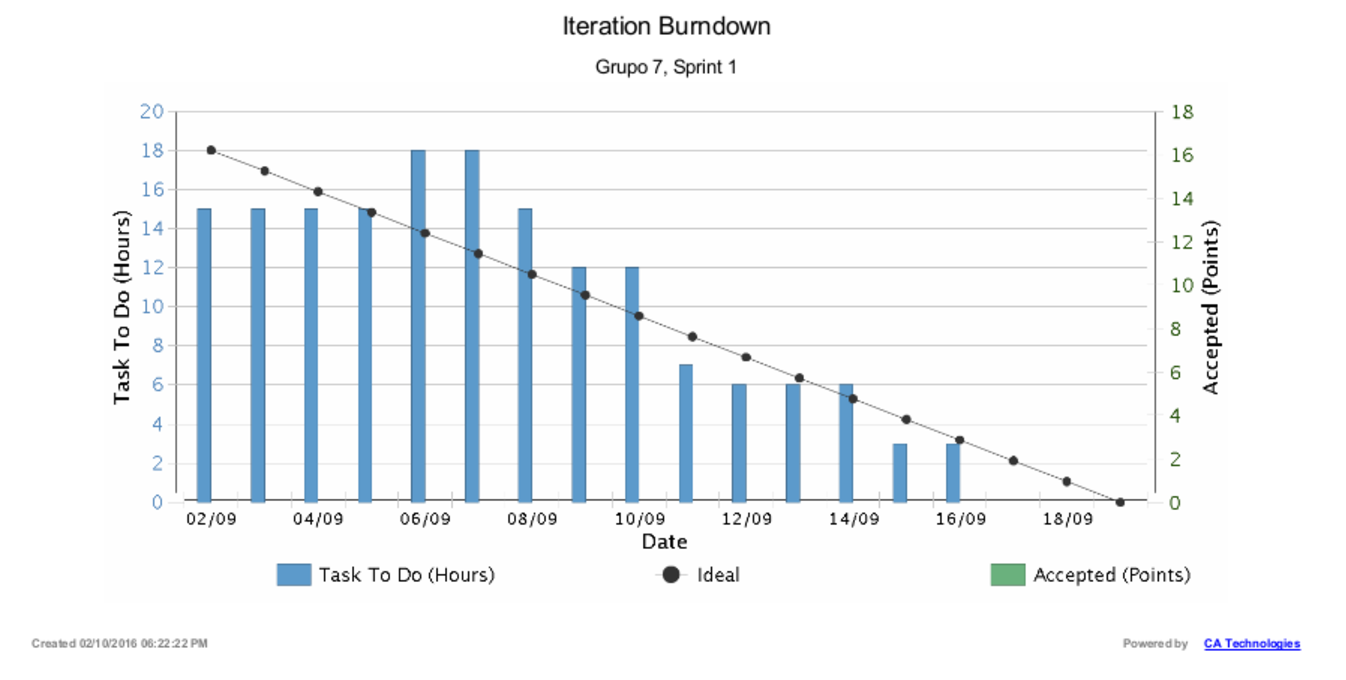
\includegraphics[width=\textwidth]{diagramas/iteration_burndown1.pdf}
  \caption{}
  \label{fig:burndown1}
\end{figure}

La subida en la cantidad de horas restantes que puede observarse el 06/09 se explica porque se nos había pasado por alto asignarle la estimación de horas a la User Story ``Vista de bar'' al momento de crearla. El 06/09 fue cuando corregimos dicho error.

\subsection{Segundo Sprint}

\subsection{Retrospectiva}